\documentclass[a4paper, 12pt]{article}
\usepackage[utf8]{inputenc}
\usepackage[english,russian]{babel}
\usepackage[warn]{mathtext}
\usepackage{graphicx}
\usepackage{float}
\restylefloat{table}
\usepackage{amsmath}
\usepackage{floatflt}
\usepackage[T2A]{fontenc}
\usepackage[left=20mm, top=20mm, right=20mm, bottom=20mm, footskip=10mm]{geometry}

\tolerance 1414
\hbadness 1414
\emergencystretch 1.5em
\hfuzz 0.3pt        % размер максимального переполнения без warning'a
\widowpenalty=10000 % запрещает одиночную строку абзаца в начале страницы
\vfuzz \hfuzz
\raggedbottom       % если на странице мало содержимого, добавить пустое место в конце, а не в середине страницы



\begin{document}

\begin{titlepage}
	\centering
	\vspace{5cm}
	{\scshape\LARGE московский физико-технический институт (национальный исследовательский университет) \par}
	\vspace{6cm}
	{\scshape\Large Лабораторная работа 3.2.5 \par}
	{\huge\bfseries Вынужденные колебания в электрическом контуре \par}
	\vspace{1cm}
	\vfill
\begin{flushright}
	{\large Б03-102}\par
	\vspace{0.3cm}
	{\LARGE Куланов Александр}
\end{flushright}
	

	\vfill


	Долгопрудный, 2022 г.
\end{titlepage}

\begin{itemize}
	\item \textbf{Цель работы:} исследование вынужденных колебаний и процессов их установления в колебательном контуре.
    \item \textbf{В работе используются:} генератор звуковых частот, вольтметр, частотомер, конденсатор, катушка индуктивности, магазин сопротивлений, осциллограф, универсальный измеритель импеданса ($LCR$-метр).
    
\end{itemize}



\section{Теоретические сведения}

Для экспериментального исследования резонансной кривой тока в последовательном колебательном контуре 
можно снять зависимость амплитуды напряжения на резситоре $R$ от частоты генератора 
(при постоянной амплитуде выходного напряжения генератора). Но импеданс этого контура включает 
в себя выходной импеданс генератора. Мы должны быть уверены, что выходной импеданс генератора 
много меньше импеданса контура и не влияет на процессы, происходящие в этом контуре.
	
	Для устранения этого влияния можно использовать схему, представленную на рисунке 
	\ref{fig:set}: синусоидальный синал с генератора подаётся на параллельный колебательный 
	контур через небольшую разделительную ёмкость $C_1$. Напряжение с ёмкости контура $C$ 
	поступает на вертикальный вход ЭО.
	
	Зависимость амплитуды этого напряжения от частоты генератора будет практически совпадать 
	с резонансной кривой для последовательного контура, если импедансы возбуждающей и измеряющей 
	цепей (сопротивления переменному току) намного превосходят импеданс самого контура вблизи 
	резонанса $Z_\text{рез} \approx L / (RC) = Q / (\Omega C)$. Разделительная ёмкость $C_1$ 
	выбирается настолько малой, что в рабочем диапазоне частот её импеданс $Z_{C_1} = 1/(\Omega C_1)$
	 много меньше импеданса контура, поэтому в цепи генератора течёт ток практически с постоянной 
	 амплитудой, а колебательный контур выполняет роль нагрузочного сопротивления, которое, в свою 
	 очередь, зависит от частоты. Поскольку в резонансе сопротивление $Z_\text{рез}$ параллельного 
	 контура максимально, то и напряжение на ёмкости $C$ (неизменный ток, умноженный на максимальное 
	 сопротивление) тоже максимально. Входное сопротивление осциллографа (измеряющей цепи) достаточно 
	 велико: $R_\text{ЭО} \approx 1 \text{МОм}$.
	
	Таким образом, при выполнении условий
	\begin{equation}
		Z_{C_1} = \frac{1}{\Omega C_1} \gg |Z| = \frac{Q}{\Omega C}, \quad R_\text{ЭО} \gg \frac{Q}{\Omega C}
	\end{equation}
	и при условии, что действительная часть импеданса катушки много меньше её мнимой части, резонансная кривая в нашем контуре бует выглядеть так же, как в последовательном: максимум амплитуды при резонансе. Ширина резонансной кривой определяет важную характеристику контура --- добротность.
	
	Добротность контура может быть определена и другими способами, например, по скорости нарастания амплитуды вынужденных колебаний при резонансе или по скорости затухания свободных колебаний. Нарастание и затухание колебаний можно наблюдать на экране осциллографа, если на контур подаются цуги --- отрезки синусоиды, разделённые интервалами, в течение которых сигнал отсутствует. Чем выше добротность, тем медленне нарастают и медленнее затухают колебания в контуре. Количественные оценки можно сделать, сли определить логарифмический декремент затухания по скорости нарастания или затухания колебаний. В условиях резонанса огибающая затухающих колебаний это перевёрнутая огибающая нарастающего участка, поэтому при расчёте логарифмического декремента по затуханию нет необходимости использовать амплитуду установившихся колебаний $U_0$, которая в контуре с высокой добротностью иногда не успевает установиться за время продолжительности цуга.


\section{Экспериментальная установка}

Схема установки представлена на рисунке \ref{fig:set}. Колебательный контур состоит из конденсатора с ёмкостью
$C$, катушки с индуктивностью $L$ и магазина сопротивлений $R$. Синусоидальный сигнал генерируется звуковым
генератором (ЗГ), а сигнал, состоящий из отрезков синусоиды (цугов), формируется цифровым генератором электрических
сигналов произвольной формы или комбинацией генератора синусоидального сигнала звукового диапазона и электронного 
реле, прерывающего сигнал с заданной периодичностью. Результирующие сигналы --- цуги или непрерывная синусоида 
--- поступают по отдельным каналам через одинаковые небольшие ёмкости $C_1$ соответственно на клеммы "цуги" и "непр."{},
смонтированные на панели "П"{}, на которой расположенны также клеммы "синхр." (синхронизация) и "$\perp$" (земля).
При подключении контура к клемме "$\perp$"{} и через амперметр $A$ к клемме "непр."{} на него подается непрерывный
сигнал --- синусоида; если контур подключен "цуги"{} и "$\perp$"{}, то на контур поступают отрезки синусоиды. 

\begin{figure}[h]
    \centering
    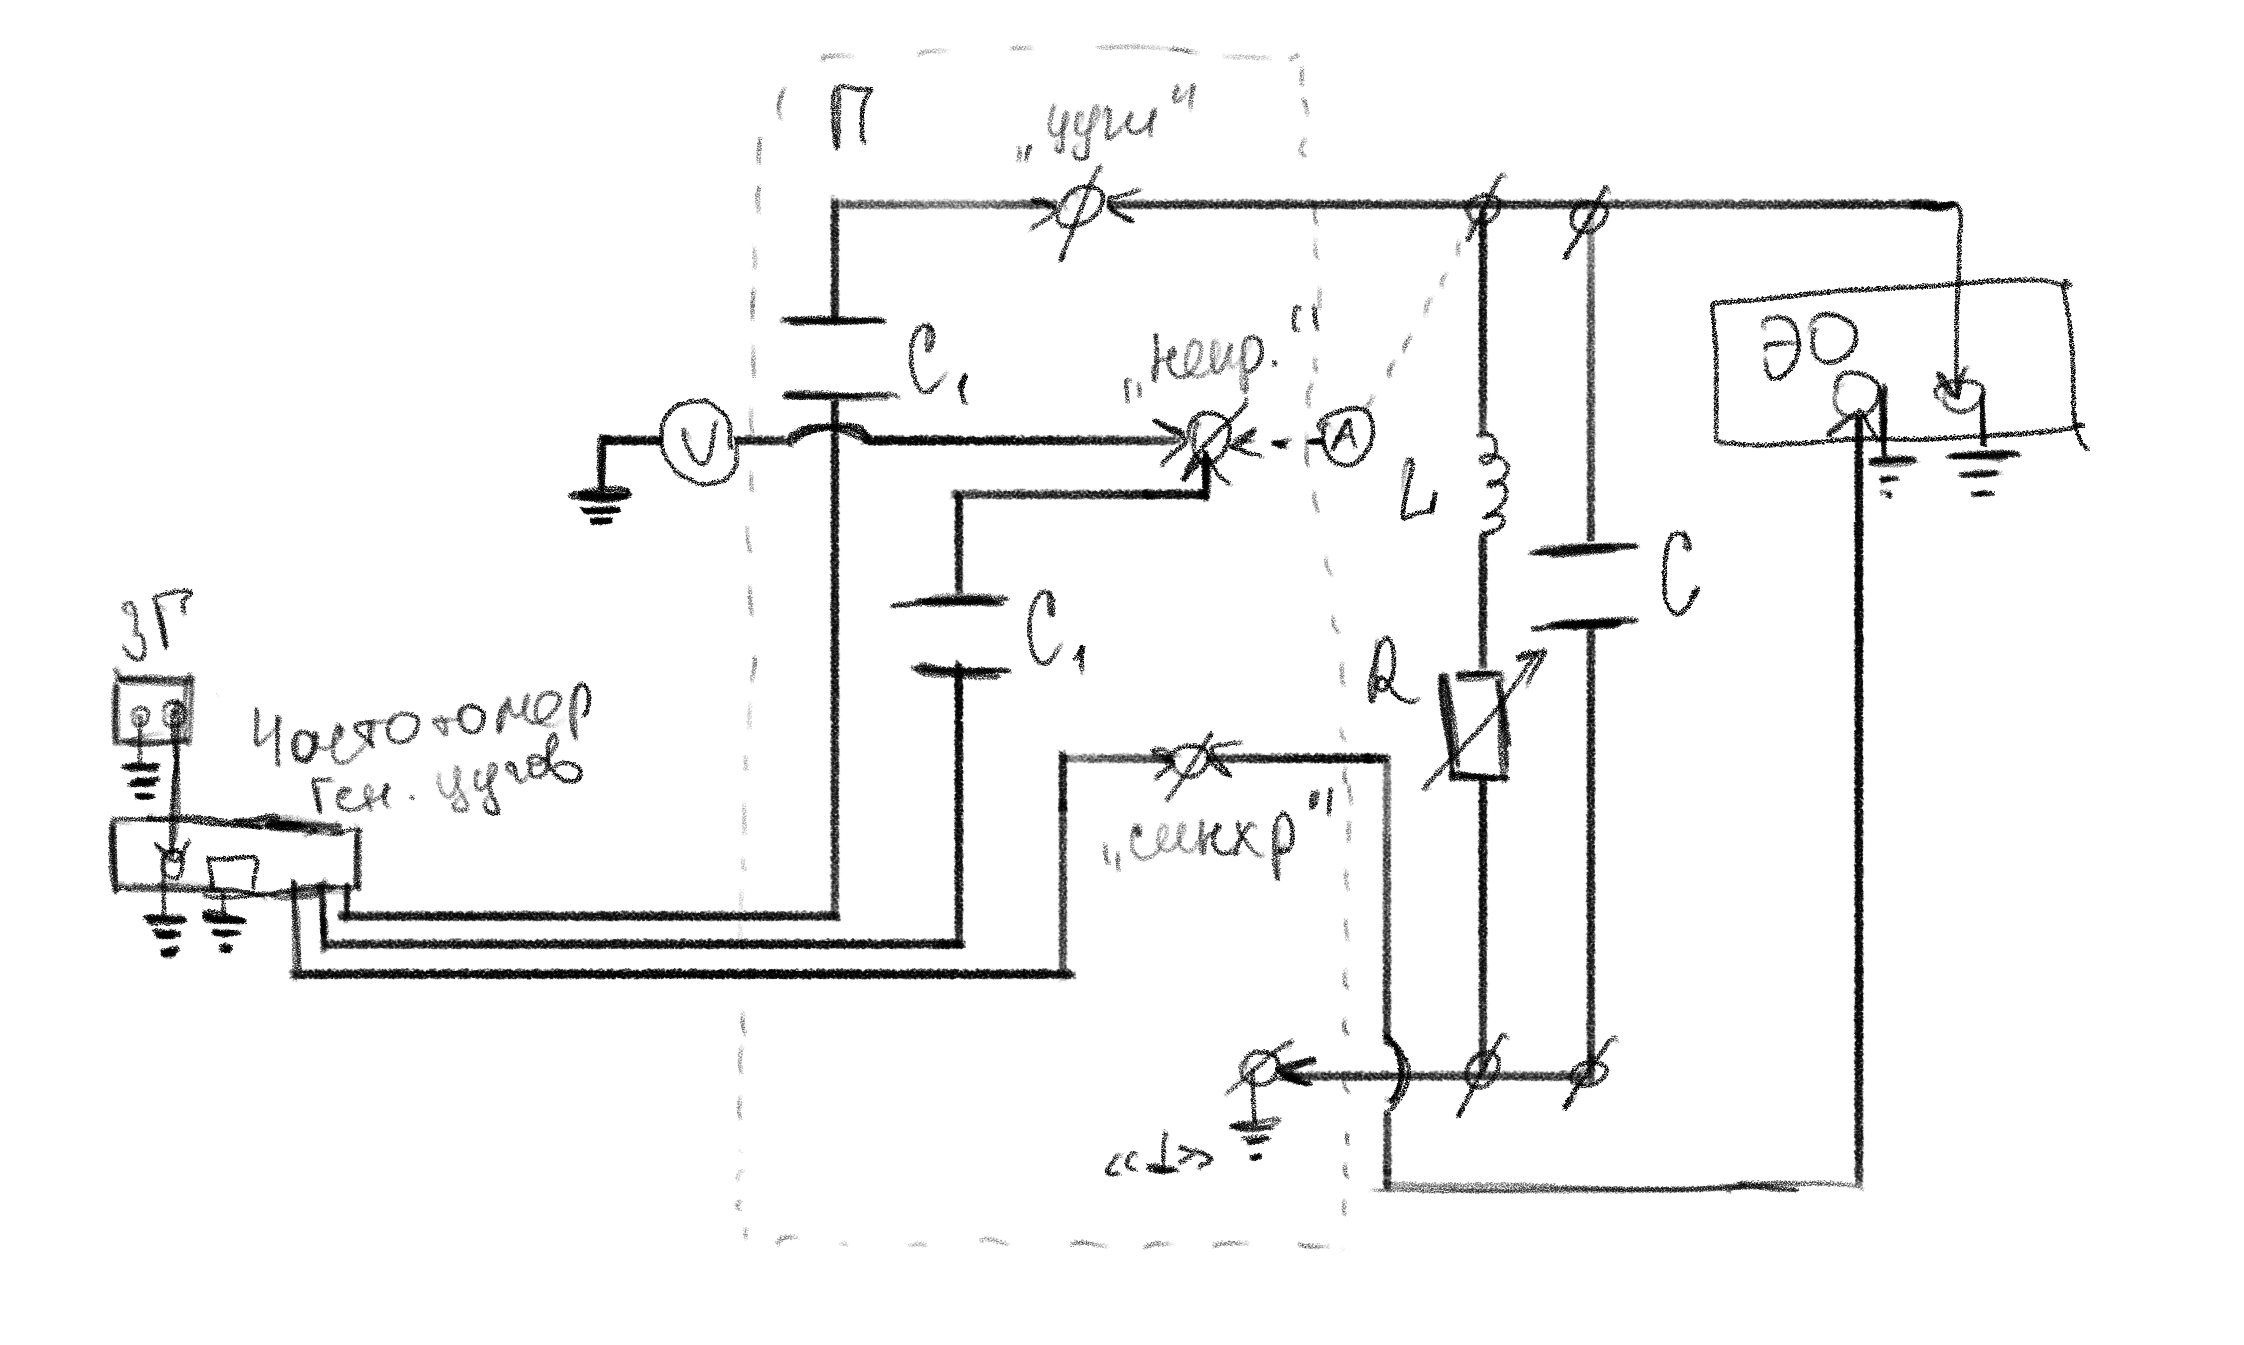
\includegraphics[width=1\textwidth]{set}
    \caption{Схема установки}
    \label{fig:set}
\end{figure}

Эффективное значение тока $I(\omega)$, текущего к контуру от генератора в режиме непрерывного сигнала, 
измеряется амперметром $A$, а соответствующее значение тока в контуре определяется по формуле $I_C(\omega) = \omega C U_C (\omega)$,
где $U_C(\omega)$ --- эффективное напряжение на конденсаторе, измеряемое вольтметром $V$.

Для визуального наблюдения за процессом колебаний напряжение с ёмкости контура $C$ подаётся на вход электронного
осциллографа. Чтобы картина на экране была устойчивой, частота развёртки осциллографа принудительно синхронизируется
с частотой повторения цугов. Для этого на генератор ЭО подаются следующие с частотой повторения цугов управляющие 
импульсы, формируемые в блоке электронного реле, клемма "синхр."{} которого смонтирована на панели "П".

Используя представленную схему в режиме непрерывного синусоидального сигнала, можно по показаниям приборов и известных
параметров элементов цепи измерить амплитудно-частотную характеристику (резонансную кривую) $I_C(\omega)$ в необходимом
диапазоне частот. Сравнивая результат измерения с теоретической кривой, можно определить характеристики контура
$\omega_m \approx \omega_0$ и $Q$.

\section{Обработка результатов}

\subsection{Метод резонансных кривых}

Данные зависимости $U$ и $I$ от частоты $\nu$ приведены в таблице \ref{tab:data}

\begin{table}[h]
	\centering
	\begin{tabular}{|ccc|ccc|}
	\hline
	\multicolumn{3}{|c|}{\textbf{R = 100 Ом}}                         & \multicolumn{3}{c|}{\textbf{R = 0 Ом}}                           \\ \hline
	\multicolumn{1}{|c|}{$\nu$, Гц} & \multicolumn{1}{c|}{U, мВ} & I, мA & \multicolumn{1}{c|}{$\nu$, Гц} & \multicolumn{1}{c|}{U, мВ} & I, мА \\ \hline
	\multicolumn{1}{|c|}{855}    & \multicolumn{1}{c|}{30}    & 22,29 & \multicolumn{1}{c|}{1338}   & \multicolumn{1}{c|}{30}    & 9,51  \\ \hline
	\multicolumn{1}{|c|}{1140}   & \multicolumn{1}{c|}{60}    & 30    & \multicolumn{1}{c|}{1441}   & \multicolumn{1}{c|}{60}    & 10,71 \\ \hline
	\multicolumn{1}{|c|}{1266}   & \multicolumn{1}{c|}{90}    & 33,73 & \multicolumn{1}{c|}{1476}   & \multicolumn{1}{c|}{90}    & 11,46 \\ \hline
	\multicolumn{1}{|c|}{1340}   & \multicolumn{1}{c|}{120}   & 35,92 & \multicolumn{1}{c|}{1497}   & \multicolumn{1}{c|}{120}   & 11,95 \\ \hline
	\multicolumn{1}{|c|}{1388}   & \multicolumn{1}{c|}{150}   & 37,44 & \multicolumn{1}{c|}{1511}   & \multicolumn{1}{c|}{150}   & 12,39 \\ \hline
	\multicolumn{1}{|c|}{1424}   & \multicolumn{1}{c|}{180}   & 38,51 & \multicolumn{1}{c|}{1520}   & \multicolumn{1}{c|}{180}   & 12,73 \\ \hline
	\multicolumn{1}{|c|}{1454}   & \multicolumn{1}{c|}{210}   & 39,31 & \multicolumn{1}{c|}{1528}   & \multicolumn{1}{c|}{210}   & 12,92 \\ \hline
	\multicolumn{1}{|c|}{1464}   & \multicolumn{1}{c|}{222}   & 39,54 & \multicolumn{1}{c|}{1535}   & \multicolumn{1}{c|}{240}   & 12,92 \\ \hline
	\multicolumn{1}{|c|}{1478}   & \multicolumn{1}{c|}{240}   & 39,83 & \multicolumn{1}{c|}{1544}   & \multicolumn{1}{c|}{270}   & 12,46 \\ \hline
	\multicolumn{1}{|c|}{1490}   & \multicolumn{1}{c|}{252}   & 39,97 & \multicolumn{1}{c|}{1556}   & \multicolumn{1}{c|}{288}   & 10,82 \\ \hline
	\multicolumn{1}{|c|}{1506}   & \multicolumn{1}{c|}{270}   & 40,05 & \multicolumn{1}{c|}{1563}   & \multicolumn{1}{c|}{270}   & 9,68  \\ \hline
	\multicolumn{1}{|c|}{1518}   & \multicolumn{1}{c|}{282}   & 40,03 & \multicolumn{1}{c|}{1571}   & \multicolumn{1}{c|}{240}   & 8,74  \\ \hline
	\multicolumn{1}{|c|}{1551}   & \multicolumn{1}{c|}{300}   & 39,6  & \multicolumn{1}{c|}{1578}   & \multicolumn{1}{c|}{210}   & 8,37  \\ \hline
	\multicolumn{1}{|c|}{1602}   & \multicolumn{1}{c|}{282}   & 39,04 & \multicolumn{1}{c|}{1587}   & \multicolumn{1}{c|}{180}   & 8,33  \\ \hline
	\multicolumn{1}{|c|}{1616}   & \multicolumn{1}{c|}{270}   & 39,1  & \multicolumn{1}{c|}{1598}   & \multicolumn{1}{c|}{150}   & 8,51  \\ \hline
	\multicolumn{1}{|c|}{1637}   & \multicolumn{1}{c|}{252}   & 39,36 & \multicolumn{1}{c|}{1614}   & \multicolumn{1}{c|}{120}   & 8,92  \\ \hline
	\multicolumn{1}{|c|}{1646}   & \multicolumn{1}{c|}{240}   & 39,59 & \multicolumn{1}{c|}{1642}   & \multicolumn{1}{c|}{90}    & 9,51  \\ \hline
	\multicolumn{1}{|c|}{1671}   & \multicolumn{1}{c|}{210}   & 40,1  & \multicolumn{1}{c|}{1697}   & \multicolumn{1}{c|}{60}    & 10,37 \\ \hline
	\multicolumn{1}{|c|}{1686}   & \multicolumn{1}{c|}{180}   & 40,49 & \multicolumn{1}{c|}{1926}   & \multicolumn{1}{c|}{30}    & 12,43 \\ \hline
	\multicolumn{1}{|c|}{1730}   & \multicolumn{1}{c|}{150}   & 41,75 & \multicolumn{1}{c|}{}       & \multicolumn{1}{c|}{}      &       \\ \hline
	\multicolumn{1}{|c|}{1906}   & \multicolumn{1}{c|}{120}   & 47,01 & \multicolumn{1}{c|}{}       & \multicolumn{1}{c|}{}      &       \\ \hline
	\multicolumn{1}{|c|}{2243}   & \multicolumn{1}{c|}{90}    & 56,06 & \multicolumn{1}{c|}{}       & \multicolumn{1}{c|}{}      &       \\ \hline
	\end{tabular}
	\caption{Данные}
	\label{tab:data}
\end{table}

Найдём собственную частоту контура:

\begin{equation}
	\nu_0 = \frac{1}{2 \pi \sqrt{L C}} = 1592 \text{ Гц}
\end{equation}

Построим графики зависимости $\frac{U}{U_m} = f(\frac{\nu}{\nu_m})$, где $U_m, \nu_m$ --- параметры при резонансе: 
рис. \ref{fig:graph}.

Далее, по графику и формуле $Q = \nu_0 / 2\Delta\nu$ определим добротность контура:

\begin{equation}
	Q_{100\Omega} = 7.34 \pm 2.1
\end{equation}
\begin{equation}
	Q_{0\Omega} = 25.45  \pm 7.2
\end{equation}

\subsection{Метод исследования затухания и установления колебаний}

Определим теперь добротность по скорости затухания колебаний. Для этого воспользуемся формулами:
\begin{equation}
	Q = \frac{\pi}{\Theta},
\end{equation}
где для нарастания колебаний
\begin{equation}
	\Theta = \frac{1}{n}\ln \left(\frac{U_{0} - U_{k}}{U_{0} - U_{k + n}}\right),
\end{equation}
а для затухания
\begin{equation}
	\Theta = \frac{1}{n}\ln \left(\frac{U_{k}}{U_{k + n}}\right),
\end{equation}
Результаты расчетов:
\begin{table}[h]
	\centering
	\begin{tabular}{|l|l|l|l|l|}
	\hline
	R, Ом & Q, возр. & $\sigma$ & Q, убыв & $\sigma$ \\ \hline
	0     & 24.2    & 8.1      & 29.3   & 7.4      \\ \hline
	100   & 5.8     & 1.8      & 6.9   & 0.8     \\ \hline
	\end{tabular}
	\caption{Добротности контуров}
	\label{tab:Qs}
\end{table}

\subsection{Теоретический метод}

Теоретически рассчитать добротность можно по формуле. Значение индуктивности определим по RLC-метру, C = 1 мкФ:
\begin{equation}
	Q = \frac{\sqrt{L}}{R\sqrt{C}}
\end{equation}
Посчитаем и занесём всё в сводную таблицу \ref{tab:itogi} (см. далее)

\section{Вывод}

В ходе работы было изучено, как узнать добротность контура тремя разными способами: методом резонансных кривых,
методом затухающих и нарастающих колебаний, и теоретическим методом.

\begin{table}[h]
	\centering
	\begin{tabular}{|l|l|l|l|l|}
	\hline
	R, Ом & Q, рез. кривые & Q, уст. колеб. & Q, затух. колеб. & Q, теор. \\ \hline
	0     & 25.4          & 24.1          & 29.3           & 32.3    \\ \hline
	100   & 7.3           & 5.8           & 6.9             & 7.6     \\ \hline
	\end{tabular}
	\caption{Сводная таблица}
	\label{tab:itogi}
\end{table}
Результаты измерения добротности колебательного контура разными методами не сошлись между собой. Вероятно, 
где-то были допущены ошибки при выполнении или при расчетах. Также, нельзя исключать наличие в контуре дополнительных
сопротивлений, ёмкостей и индуктивностей.

\section{Приложение}

\begin{figure}[H]
    \centering
    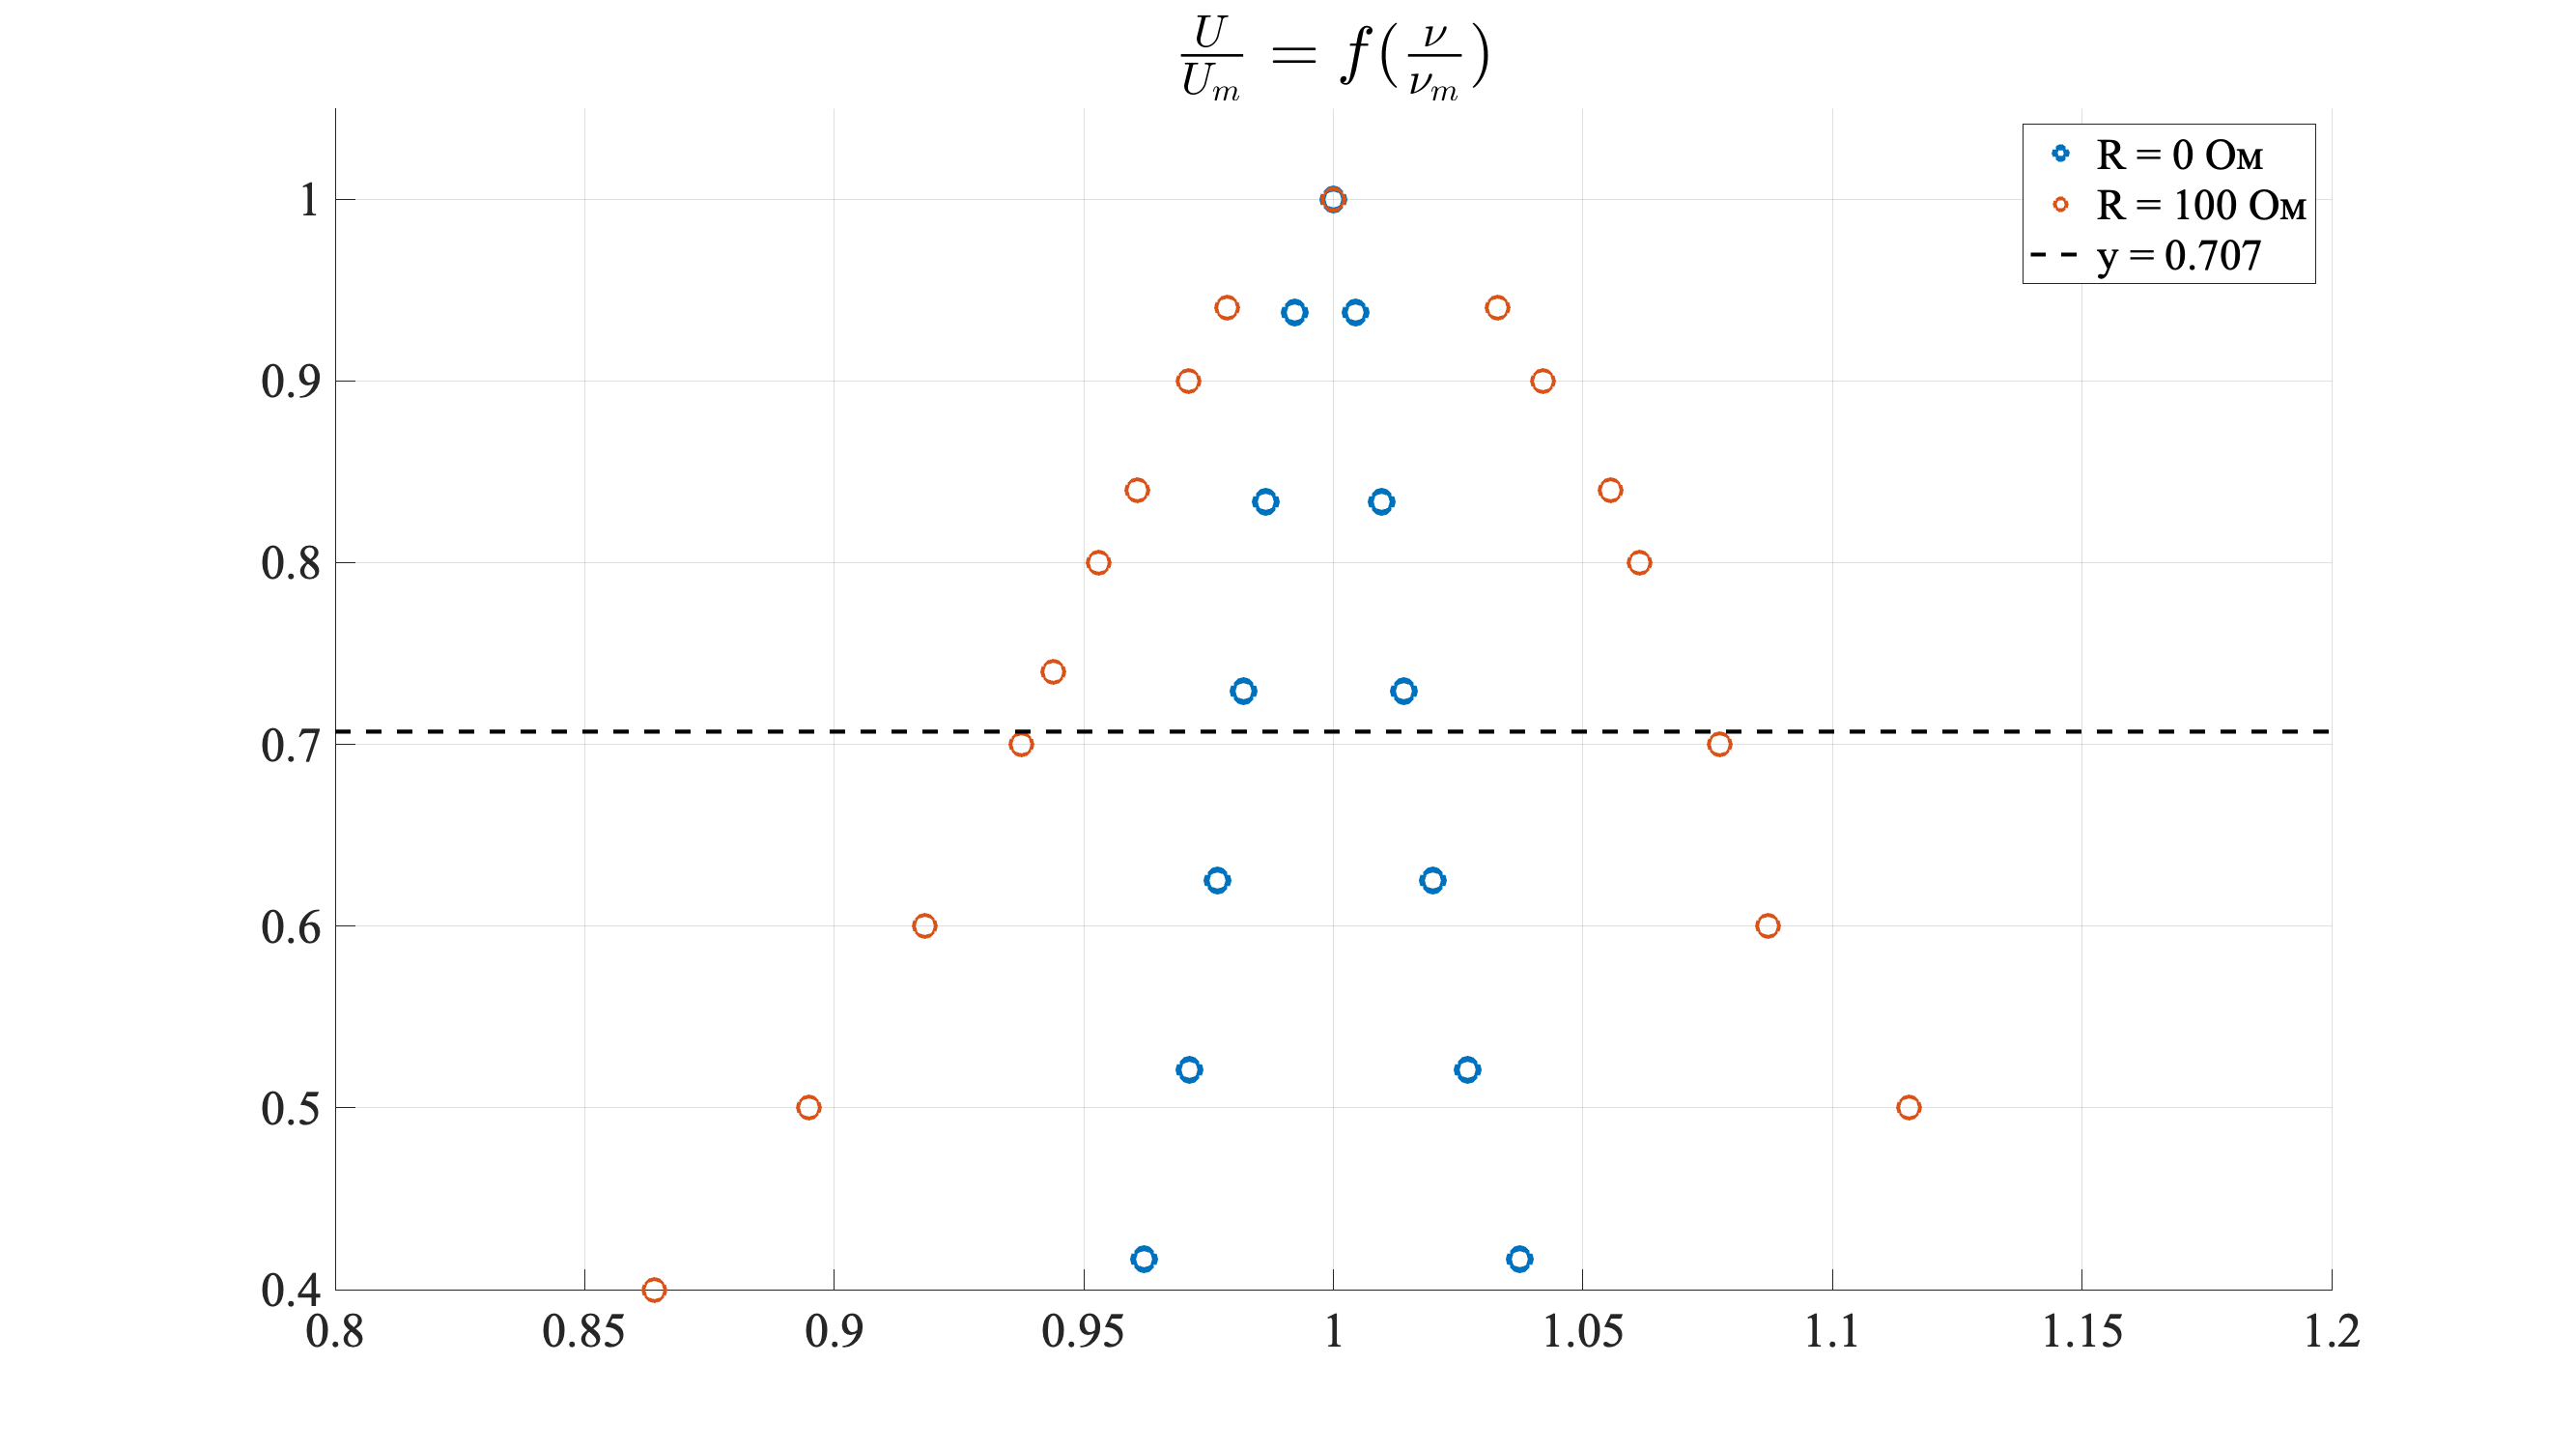
\includegraphics[width=1\textwidth]{plot}
    \caption{$\frac{U}{U_m} = f(\frac{\nu}{\nu_m})$}
    \label{fig:graph}
\end{figure}

\end{document}